

\section{Thermal Transport Analysis}

For dynamic thermal capacity analysis in Cyder, a transient model utilizes a 
linear approximation of heat based capacity quickly for each 
arbitrary waste stream offered to the repository. This relies on a thermal reference database of repository heat 
evolution curves covering the thermal coefficient range of the main geologies of 
interest and over a range of realistic waste package spacings. 
\subsection{Supporting Thermal Response Dataset}
To support this calculation in \Cyder , a reference data set of temperature change 
curves was calculated. Repeated runs of a detailed analytic model over the range of values in Table 
\ref{tab:thermal_cases} determined \gls{STC} values over a range of thermal 
heat limit radii, $r_{lim}$, thermal diffusivity values, $\alpha_{th}$,
thermal conductivity values, $K_{th}$ and waste package spacings, $S$. Linear 
interpolation across the discrete parameter space provides a simple thermal 
reference dataset for use in \Cyder .

\begin{table}[ht!]
\centering
\footnotesize{
\begin{tabular}{|l|l|l|r|}
\multicolumn{4}{c}{\textbf{Thermal Cases}}\\
\hline
\textbf{Parameter} & \textbf{Symbol} & \textbf{Units} & \textbf{Value Range} \\
\hline
Diffusivity & $\alpha_{th}$ & $[m^2\cdot s^{-1}]$ & $1.0\times10^{-7}$\\
 & & & $2.0\times10^{-7}$\\
 & & & $3.0\times10^{-7}$\\
 & & & $4.0\times10^{-7}$\\
 & & & $5.0\times10^{-7}$\\
 & & & $6.0\times10^{-7}$\\
 & & & $7.0\times10^{-7}$\\
 & & & $8.0\times10^{-7}$\\
 & & & $9.0\times10^{-7}$\\
 & & & $1.0\times10^{-6}$\\
 & & & $2.0\times10^{-6}$\\
 & & & $3.0\times10^{-6}$\\
\hline
Conductivity & $K_{th}$     & $[W\cdot m^{-1} \cdot K^{-1}]$  & $0.1, 0.5, 1, 1.5, 2, 2.5, 3, 3.5, 4, 4.5 $ \\
\hline
Spacing & $S$ & $[m]$ & 2, 5, 10, 15, 20, 25, 50 \\
\hline
Radius & $r_{lim}$ & $[m]$ & 0.1, 0.25, 0.5, 1, 2, 5 \\
\hline
Isotope & $i$ & $[-]$ & $^{241,243}Am,$  \\
        & & & $^{242,243,244,245,246}Cm,$  \\
        & & & $^{238,240,241,242}Pu$  \\
        & & & $^{134,135,137}Cs$  \\
        & & & $^{90}Sr$  \\
\hline
\end{tabular}
\caption{A thermal reference dataset of \gls{STC} values as a function of each of these parameters was generated by repeated parameterized runs of the LLNL 
MathCAD model\cite{greenberg_application_2012, greenberg_investigations_2012}.}
\label{tab:thermal_cases}
}
\end{table}



The analytic model used to populate the reference dataset was created at 
\gls{LLNL} for the \gls{UFD} campaign. In this tool, heat limited thermal 
response is calculated analytically for each geology, for many waste package 
loading densities, and for many fuel cycle options \cite{hardin_generic_2011, 
greenberg_investigations_2012, greenberg_application_2012}. It employs an 
analytic model from Carslaw and Jaeger and is implemented in MathCAD 
\cite{carslaw_conduction_1959, ptc_mathcad_2010}.  The integral solver in the 
MathCAD toolset is the primary calculation engine for the analytic MathCAD 
thermal model, which relies on superposition of point, finite-line, and line 
source integral solutions.  

%The transient state of the temperature at the calculation radius is found with a convolution of the transient far field solution with the steady state near field solution.  The process is then iterated with a one year resolution in order to arrive at a temperature evolution over the lifetime of the repository. 
%
%In a two dimensional grid of waste packages, the central package is represented by the finite line solution

Figure \ref{fig:CmScaling} demonstrates the scaling of an STC curve according to 
equation \eqref{STC} to represent the heat from $25.9g$ of initial $^{242}Cm$ using 
the reference data set. 

\begin{figure}[h!]
\begin{center}
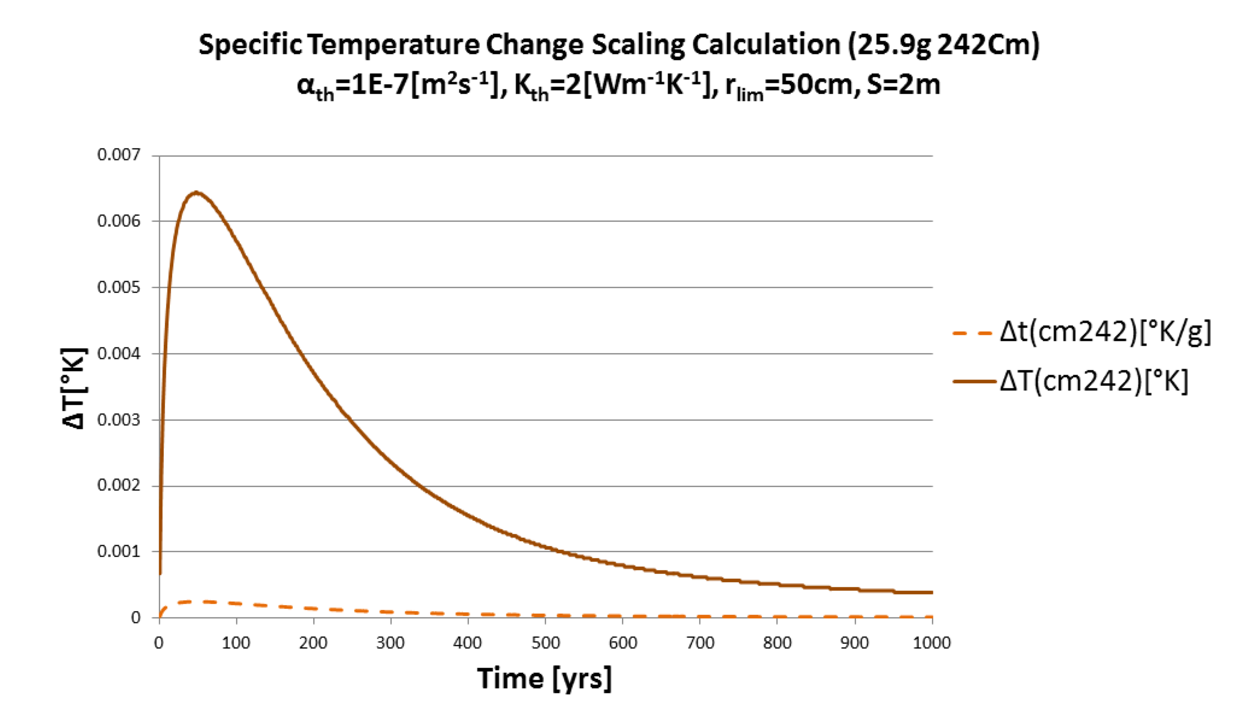
\includegraphics[width=\columnwidth]{./thermal_models/CmScaling.eps}
\end{center}
\caption{As a demonstration of the calculation procedure, the temperature change 
  curve for one initial gram of $^{242}Cm$ and is scaled to represent $25.9g$, 
  approximately the $^{242}Cm$ inventory per MTHM in 51GWd burnup UOX PWR fuel. }
\label{fig:CmScaling}
\end{figure}


The supporting database was limited to some primary heat contributing isotopes 
present in traditional spent nuclear fuel, $H$, 
such that the superposition in equation \eqref{superposition} becomes 

\begin{align}
\Delta T (r_{lim},S,K_{th},\alpha_{th})&\sim \sum_{i\in H} m_i \Delta t_i(r_{lim},S,K_{th},\alpha_{th})
\label{superposition_approx}
\intertext{where}
H &= \mbox{ set of high heat isotopes }[-]\nonumber\\
S &= \mbox{ uniform waste package spacing } [m]\nonumber\\
K_{th} &= \mbox{ thermal conductivity } [W\cdot m^{-1}\cdot K^{-1}]\nonumber\\
\alpha_{th} &= \mbox{ thermal diffusivity } [m^2\cdot s^{-1}]\nonumber\\
\end{align}

The use of this superposition is demonstrated in Figure 
\ref{fig:CmSuperposition}.

\begin{figure}[ht!]
\begin{center}
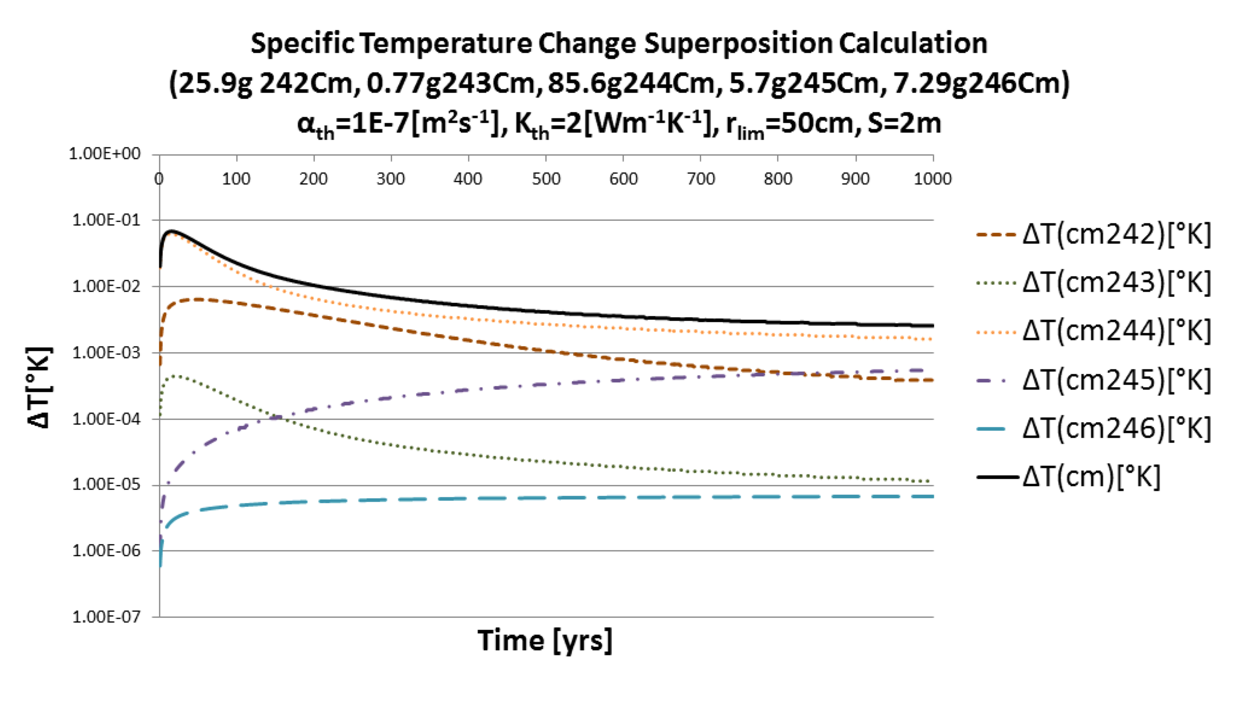
\includegraphics[width=\columnwidth]{./thermal_models/CmSuperposition.eps}
\end{center}
\caption{As a demonstration of the calculation procedure, scaled temperature change 
  curves for five curium isotopes are superimposed to achieve a total temperature 
change (note log scale).}
\label{fig:CmSuperposition}
\end{figure}

%\begin{align}
%  T_{line}(t,x,y,z) &= \frac{1}{8\pi K_{th}} 
%  \bigintsss_0^t\!\frac{q_L(t')}{t-t'}e^{ \frac{-\left(x^2 + z^2\right)}{4\alpha 
%  (t-t')} }\nonumber\\ &\cdot\left[ \erf{\left[ \frac{1}{2} \frac{\left( y + 
%  \frac{L}{2} \right)}{\sqrt{\alpha(t-t')}}  \right]} - \erf{\left[ \frac{1}{2} 
%  \frac{\left( y - \frac{L}{2} \right)}{\sqrt{\alpha(t-t')}}  \right]} 
%  \right]\,\mathrm{dt'},
%  \label{line}
%  \intertext{adjacent packages within the central tunnel are represented by the 
%  point source solution }
%  T_{point}(t,r) &= 
%  \frac{1}{8K_{th}\sqrt{\alpha}\pi^{\frac{3}{2}}}\bigintsss_0^{-t}\!\frac{q(t')}{(t-t')^{\frac{3}{2}}}e^{\frac{-r^2}{4\alpha(t-t')}}\,\mathrm{dt'},
%  \label{point}
%  \intertext{and adjacent disposal tunnels are represented by infinite line 
%  source solutions}
%  T_{\infty line}(t,x,z) &= \frac{1}{4\pi K_{th}} 
%  \bigintsss_0^t\!\frac{q_L(t')}{t-t'}e^{ \frac{-\left(x^2 + z^2\right)}{4\alpha 
%  (t-t')} }
%  \intertext{in infinite homogeneous media, where}
%  \label{infline}
%  \alpha &= ~~\mbox{thermal diffusivity } [m^2\cdot s^{-1}]\nonumber\\
%  q(t) &= ~~\mbox{point heat source} [W]\nonumber\\
%  \intertext{and}
%  q_L(t) &= ~~\mbox{linear heat source} [W\cdot m^{-1}]\nonumber
%\end{align}
%Superimposed point and line source solutions allow for a notion of the 
%repository layout to be modeled in the host rock.

\subsection{Thermal Transport Validation}\label{sec:thermal_benchmarks}

The results here provide an overview of the relative importance of thermal
parameters that that affect the repository capacity of simplified generic
disposal concept in various geologic media where conduction is the dominant
heat transfer mode. The applicability of this sensitivity analysis is thus
restricted to enclosed, backfilled concepts.  

\subsection{Parametric Domain}

Sensitivity analyses were conducted which span the parametric range of values 
generated by the reference specific temperature change database and described 
in Table \ref{tab:thermal_cases}.  

These values were selected to provide detail in the near field and at values of
$\alpha_{th}$ and $K_{th}$ in the three host media under consideration in this
work.

\subsection{Approach}

% used existing gdsms 
This analysis utilized the \gls{LLNL} semi-analytic MathCAD model utilized to 
derive supporting data and to validate behaviro within the \Cyder STC model. It 
performs detailed calculations of the conductive thermal transport in a generic 
repository concept with a gridded layout.  

It relies on the thermal diffusivity, $\alpha_{th}$ and conductivity $K_{th}$ of 
the material as well as the waste package spacing, $S$, and thermally limiting 
radius, $r_{lim}$. Finally, it relies on the \gls{STC} data calculated with the 
semi-analytic model based on the decay heat profiles of the emplace wastes, $Q$. 
The essential decay heat profiles, $Q$, were retrieved from a \gls{UFD} database 
provided by Carter et al. \cite{carter_fuel_2011}.



%\input{./thermal_demonstration/isotopics/isotopics}


\begin{frame}[ctb!]
\frametitle{LLNL Model Thermal Conductivity Sensitivity}

\begin{figure}[htbp!]
\begin{center}
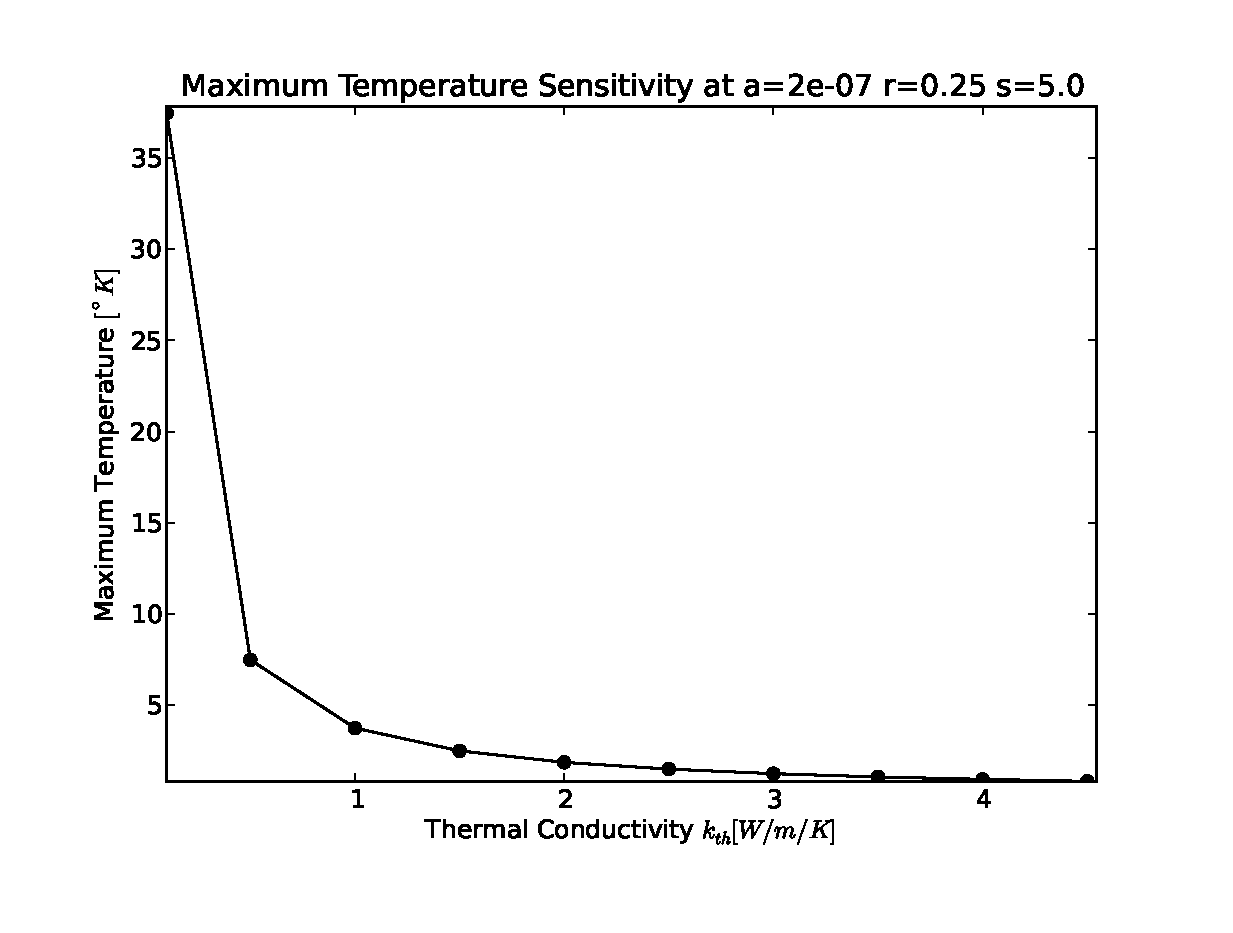
\includegraphics[height=0.7\textheight]{./thermal_demonstration/conductivity/conductivity.eps}
\end{center}
\caption[$K_{th}$ Sensitivity in LLNL Model]{Increased thermal conductivity decreases thermal energy deposition 
(here represented by STC) in the near field (here $r_{calc} = 0.5m$).}
\label{fig:Cm242Kth_alpha_low}
\end{figure}

\end{frame}


\begin{frame}[ctb!]
\frametitle{Cyder Thermal Conductivity Sensitivity}
\begin{figure}[htbp!]
\begin{center}
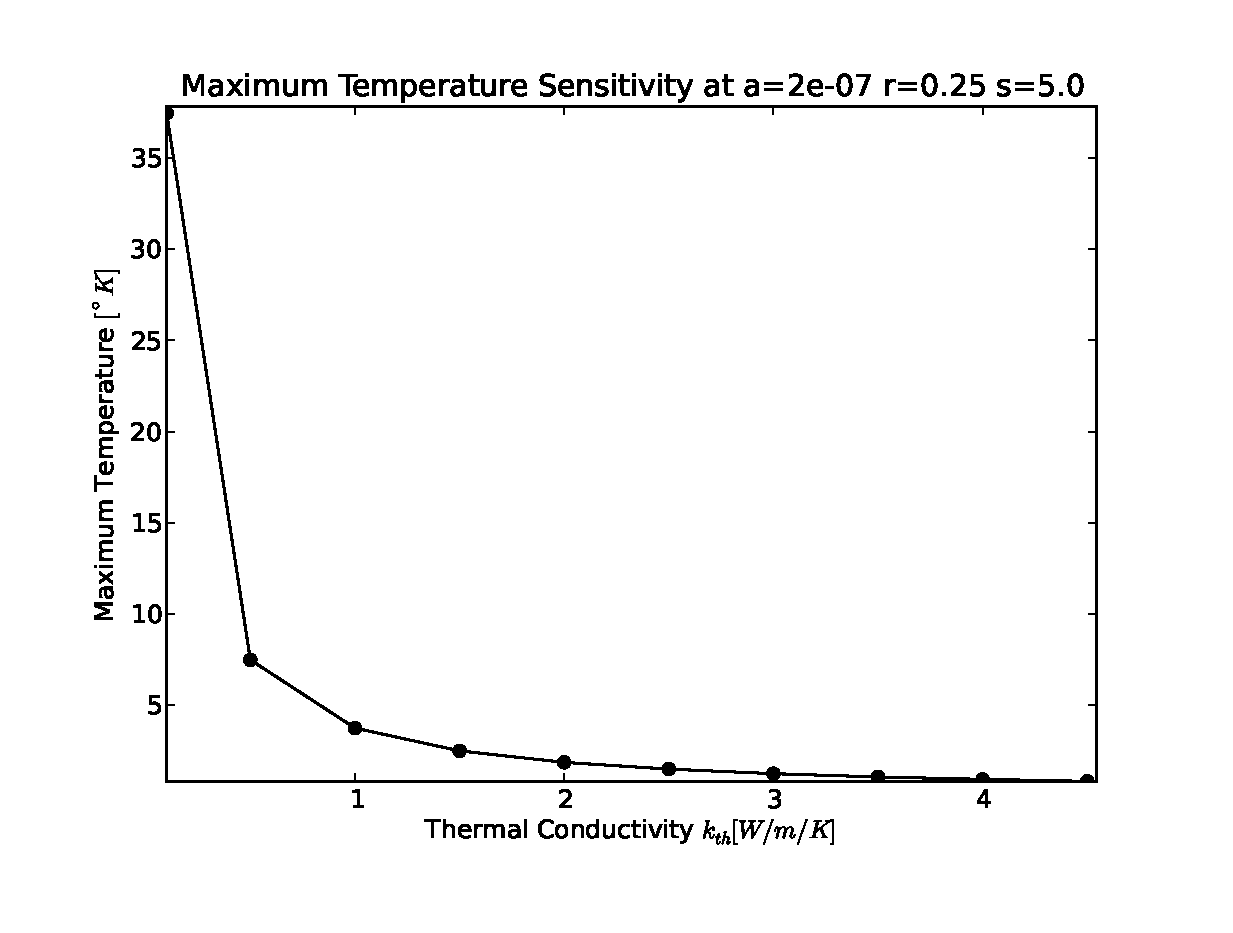
\includegraphics[height=0.7\textheight]{./thermal_demonstration/conductivity/conductivity.eps}
\end{center}
\caption[$K_{th}$ Sensitivity in Cyder]
{Cyder results agree with those of the LLNL model. Increased $K_{th}$ decreases 
thermal energy deposition at the limiting radius. The above example thermal 
profile results from 10kg of $^{242}Cm$, $\alpha_{th}=$, $s=$, and $r_{lim}=$.}
\label{fig:kr}
\end{figure}
\end{frame}

%\begin{frame}[ctb!]
%\frametitle{Cyder Thermal Conductivity and Limiting Radius Sensitivity}
%\begin{figure}[htbp!]
%\begin{center}
%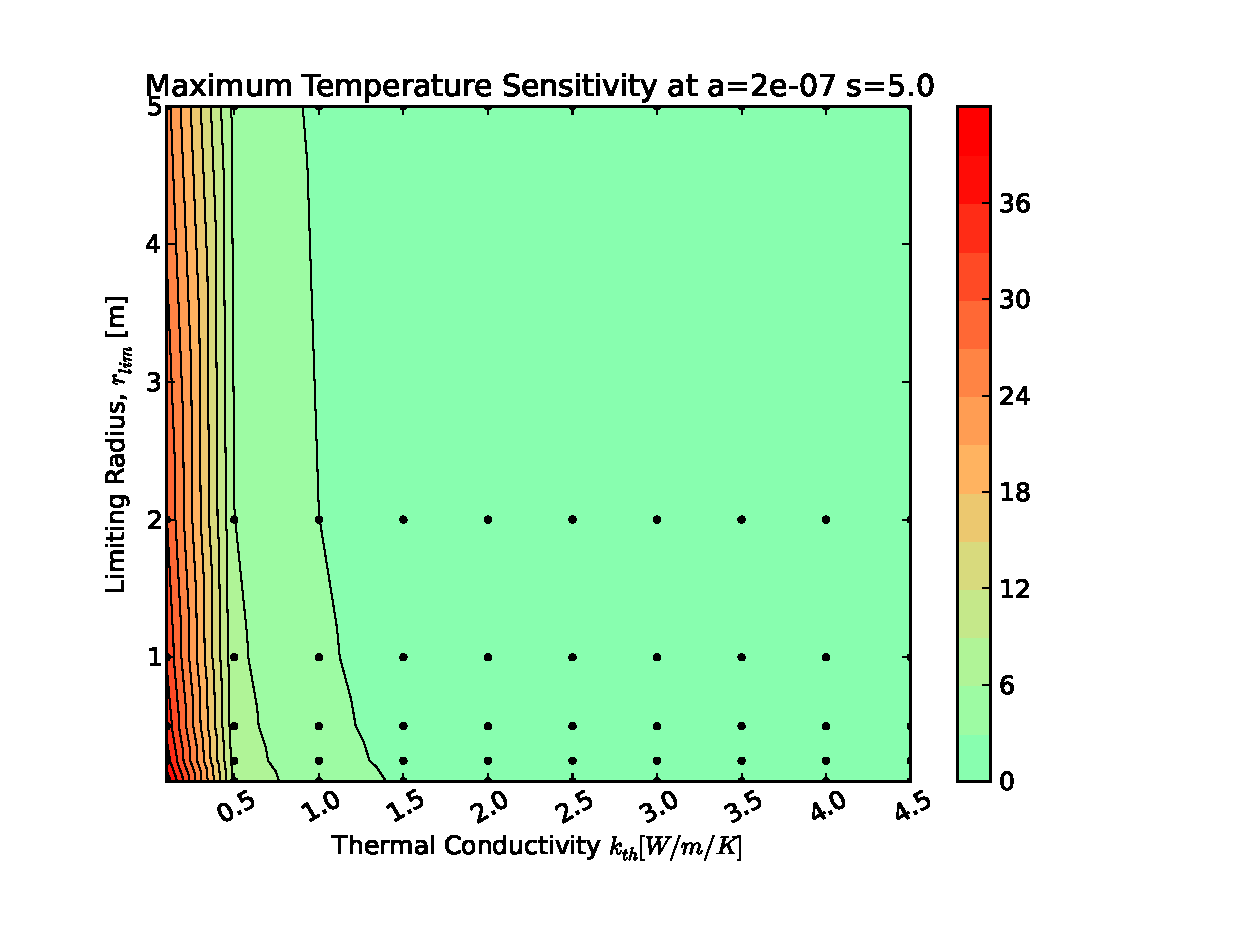
\includegraphics[height=0.7\textheight]{./thermal_demonstration/conductivity/kr.eps}
%\end{center}
%\caption[$K_{th}$ vs. $r_{lim}$ Sensitivity in Cyder]
%{Cyder results agree with 
%those of the LLNL model. The importance of the limiting radius decreases with 
%increased $K_{th}$. The above example thermal profile results from 10kg of 
%$^{242}Cm$}
%\label{fig:kr}
%\end{figure}
%\end{frame}


%\begin{frame}[ctb!]
%\frametitle{Cyder Thermal Conductivity and Limiting Radius Sensitivity}
%\begin{figure}[htbp!]
%\begin{center}
%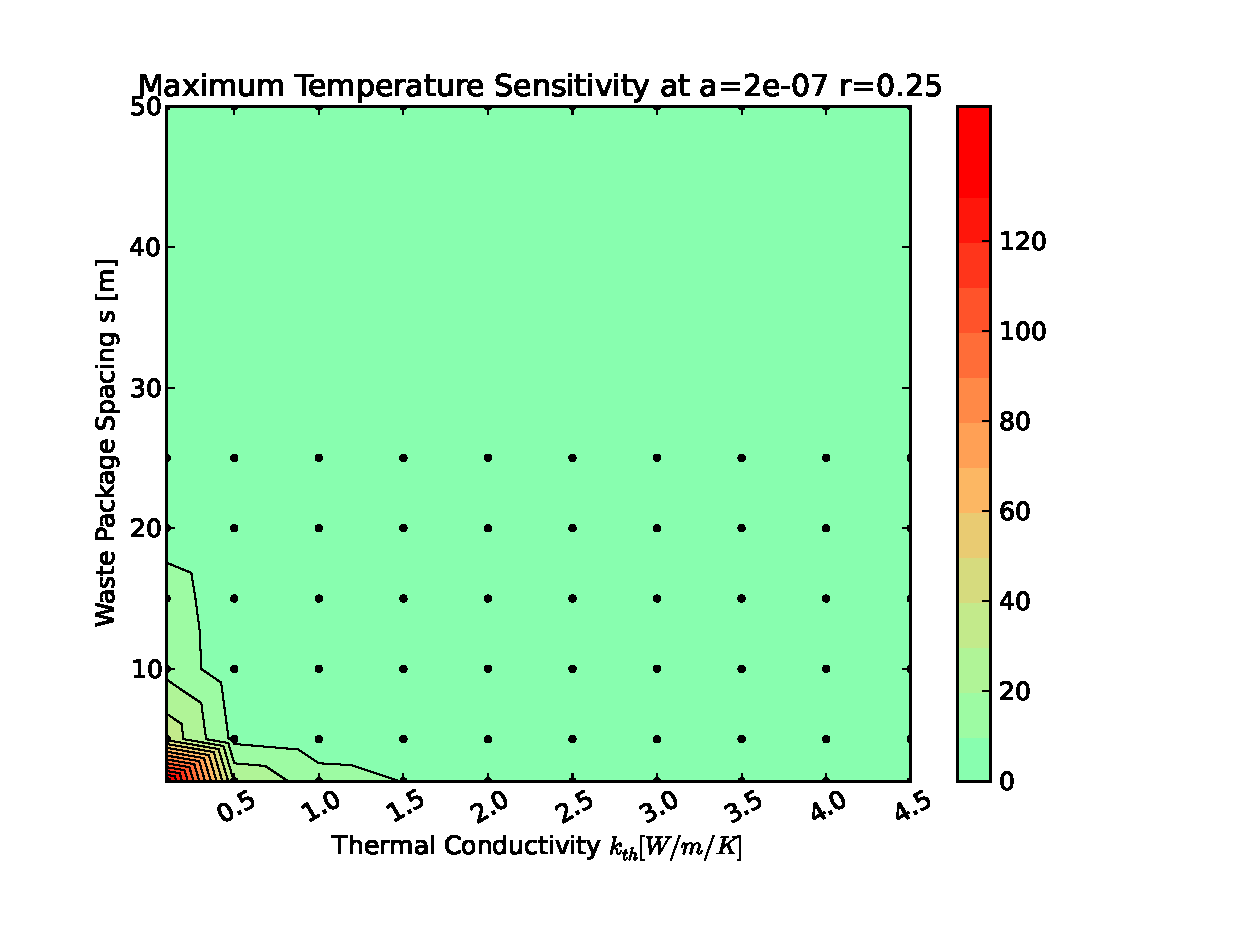
\includegraphics[height=0.7\textheight]{./thermal_demonstration/conductivity/ks.eps}
%\end{center}
%\caption[$K_{th}$ vs. Waste Package Spacing Sensitivity in Cyder]{Cyder results agree with 
%those of the LLNL model. The importance of the limiting radius decreases with 
%increased $K_{th}$. The above example thermal profile results from 10kg of 
%$^{242}Cm$}
%\label{fig:ks}
%\end{figure}
%\end{frame}


\begin{frame}[ctb!]
\frametitle{LLNL Model Thermal Diffusivity Sensitivity}
\begin{figure}[htbp!]
\begin{center}
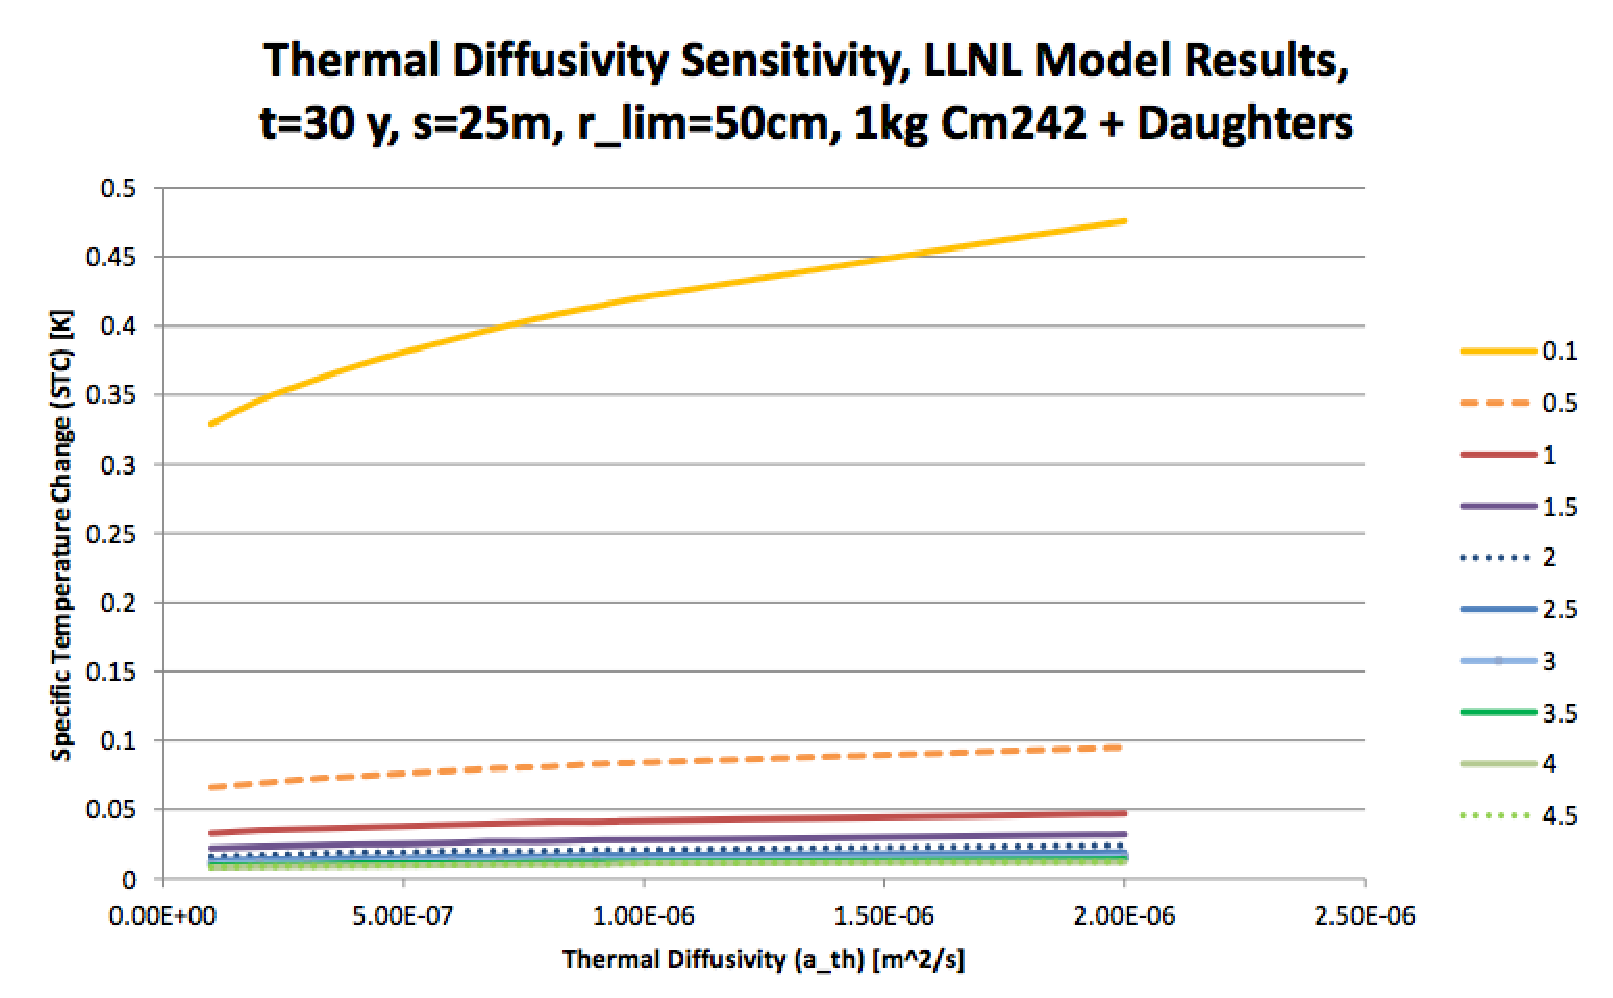
\includegraphics[height=0.7\textheight]{./thermal_demonstration/diffusivity/diffusivity.eps}
\end{center}
\caption[$K_{th}$ Sensitivity to $\alpha_{th}$]{Increased thermal 
diffusivity decreases temperature change (here represented by STC) at the 
limiting radius (here $r_{calc} = 0.5m$).}
\label{fig:Cm242alpha_kth_low}
\end{figure}
\end{frame}

\begin{frame}[ctb!]
\frametitle{Cyder Thermal Diffusivity Sensitivity}
\begin{figure}[htbp!]
\begin{center}
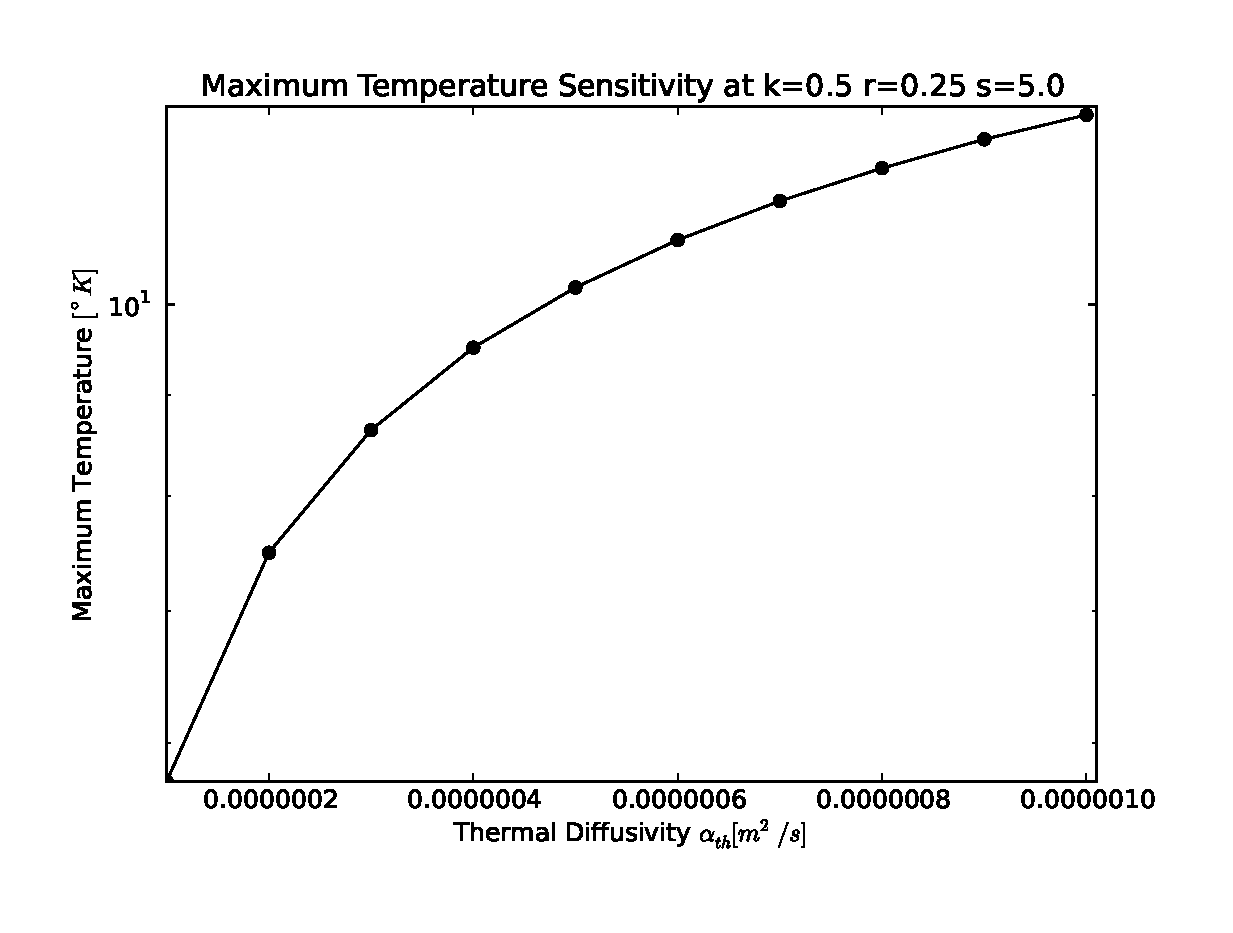
\includegraphics[height=0.7\textheight]{./thermal_demonstration/diffusivity/diffusivity_cyder.eps}
\caption[$\alpha_{th}$ Sensitivity in Cyder]{Cyder trends agree with those of 
the LLNL model, in which increased thermal diffusivity results in reduced 
temperature change at the limiting radius. The above example thermal profile 
results from 10kg of $^{242}Cm$.} 
\label{fig:ar}
\end{center}
\end{figure}
\end{frame}

%\begin{frame}[ctb!]
%\frametitle{Cyder Thermal Diffusivity and Conductivity Sensitivity}
%\begin{figure}[htbp!]
%\begin{center}
%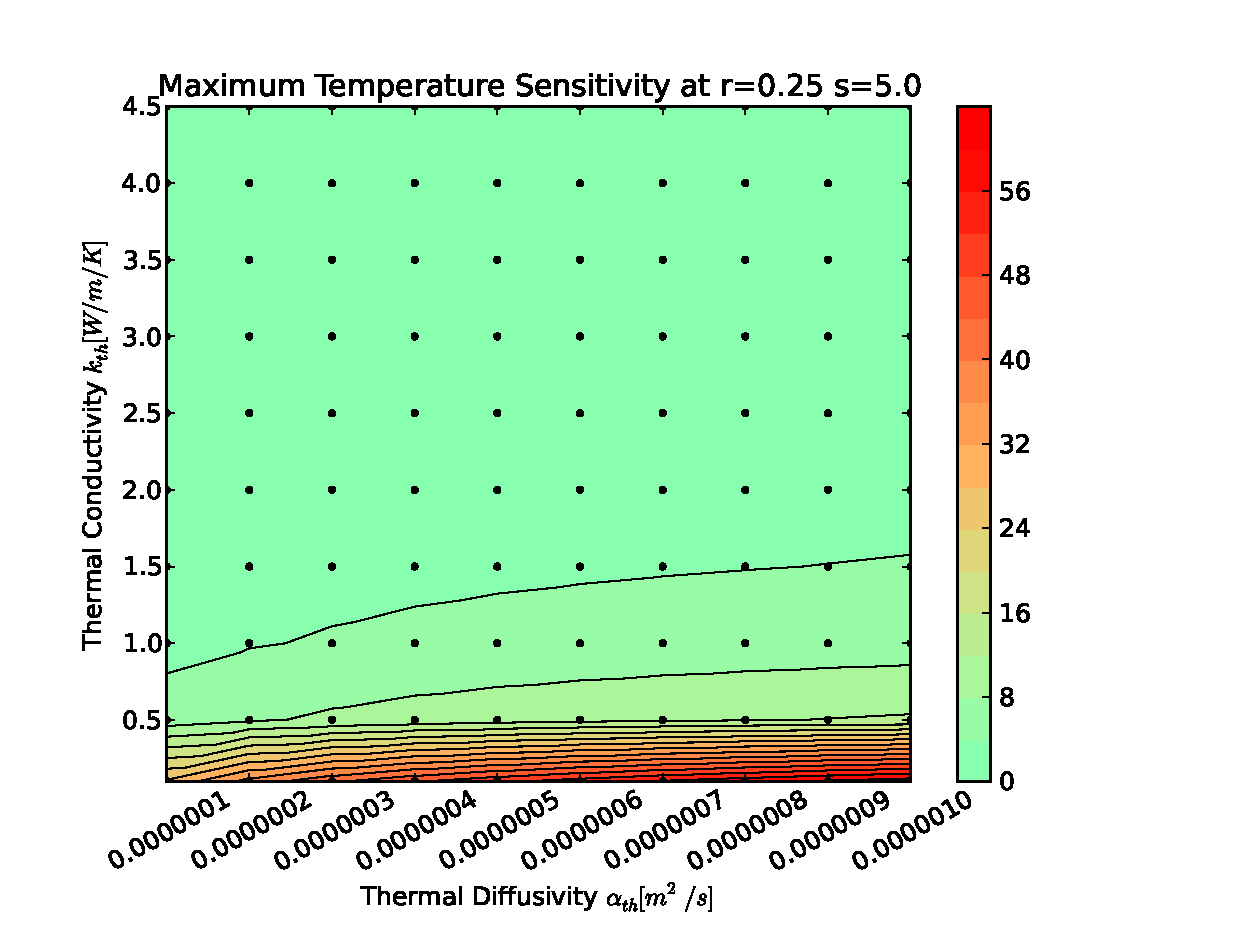
\includegraphics[height=0.7\textheight]{./thermal_demonstration/diffusivity/ak.eps}
%\caption[$\alpha_{th}$ vs. $K_{th}$ Sensitivity in Cyder]{Cyder trends agree 
%with those of the LLNL model, in which increased thermal diffusivity results in 
%decreased thermal depsoition in the near field. The above example thermal 
%profile results from 10kg of $^{242}Cm$.} 
%\label{fig:ar}
%\end{center}
%\end{figure}
%\end{frame}
%
%\begin{frame}[ctb!]
%\frametitle{Cyder Thermal Diffusivity and Limiting Radius Sensitivity}
%\begin{figure}[htbp!]
%\begin{center}
%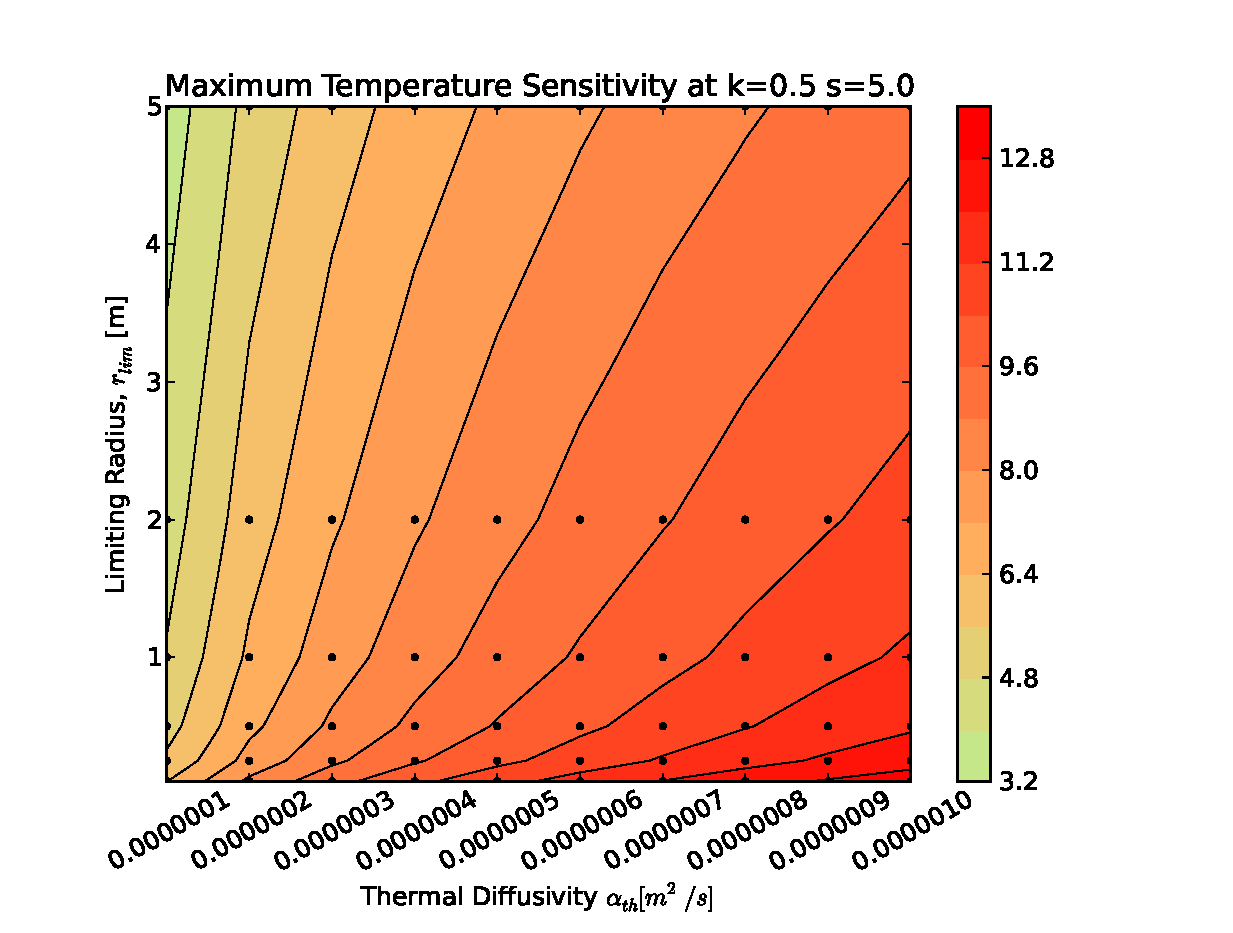
\includegraphics[height=0.7\textheight]{./thermal_demonstration/diffusivity/ar.eps}
%\end{center}
%\caption[$\alpha_{th}$ vs. $r_{lim}$ Sensitivity in Cyder]
%{Cyder trends agree with those of the LLNL model. The importance of the 
%limiting radius decreases with increased $K_{th}$. The above example thermal 
%profile results from 10kg of $^{242}Cm$.}
%\label{fig:ak}
%\end{figure}
%\end{frame}
%

\subsection{Waste Package Spacing Sensitivity Validation}\label{sec:spacing}
The waste package spacing, $s$ of geologic repository concept effects the areal 
decay heat burden in the repository and has a strong effect on the thermal 
energy deposited per unit area in the medium. 

\subsubsection{LLNL Model Results}

In the creation of the \gls{STC} database, the waste package spacing was varied 
across a number of values for each isotope, $i$, limiting 
radius $r_{calc}$, thermal diffusivity $\alpha_{th}$, and thermal conductivity $K_{th}$, considered.  By 
varying the waste package spacing of the geometric layout from $0.1-5 [m]$
this sensitivity analysis succeeds in capturing the domain of 
waste package spacings present in geologic repository concepts under 
consideration. 

\begin{figure}[htbp!]
\begin{center}
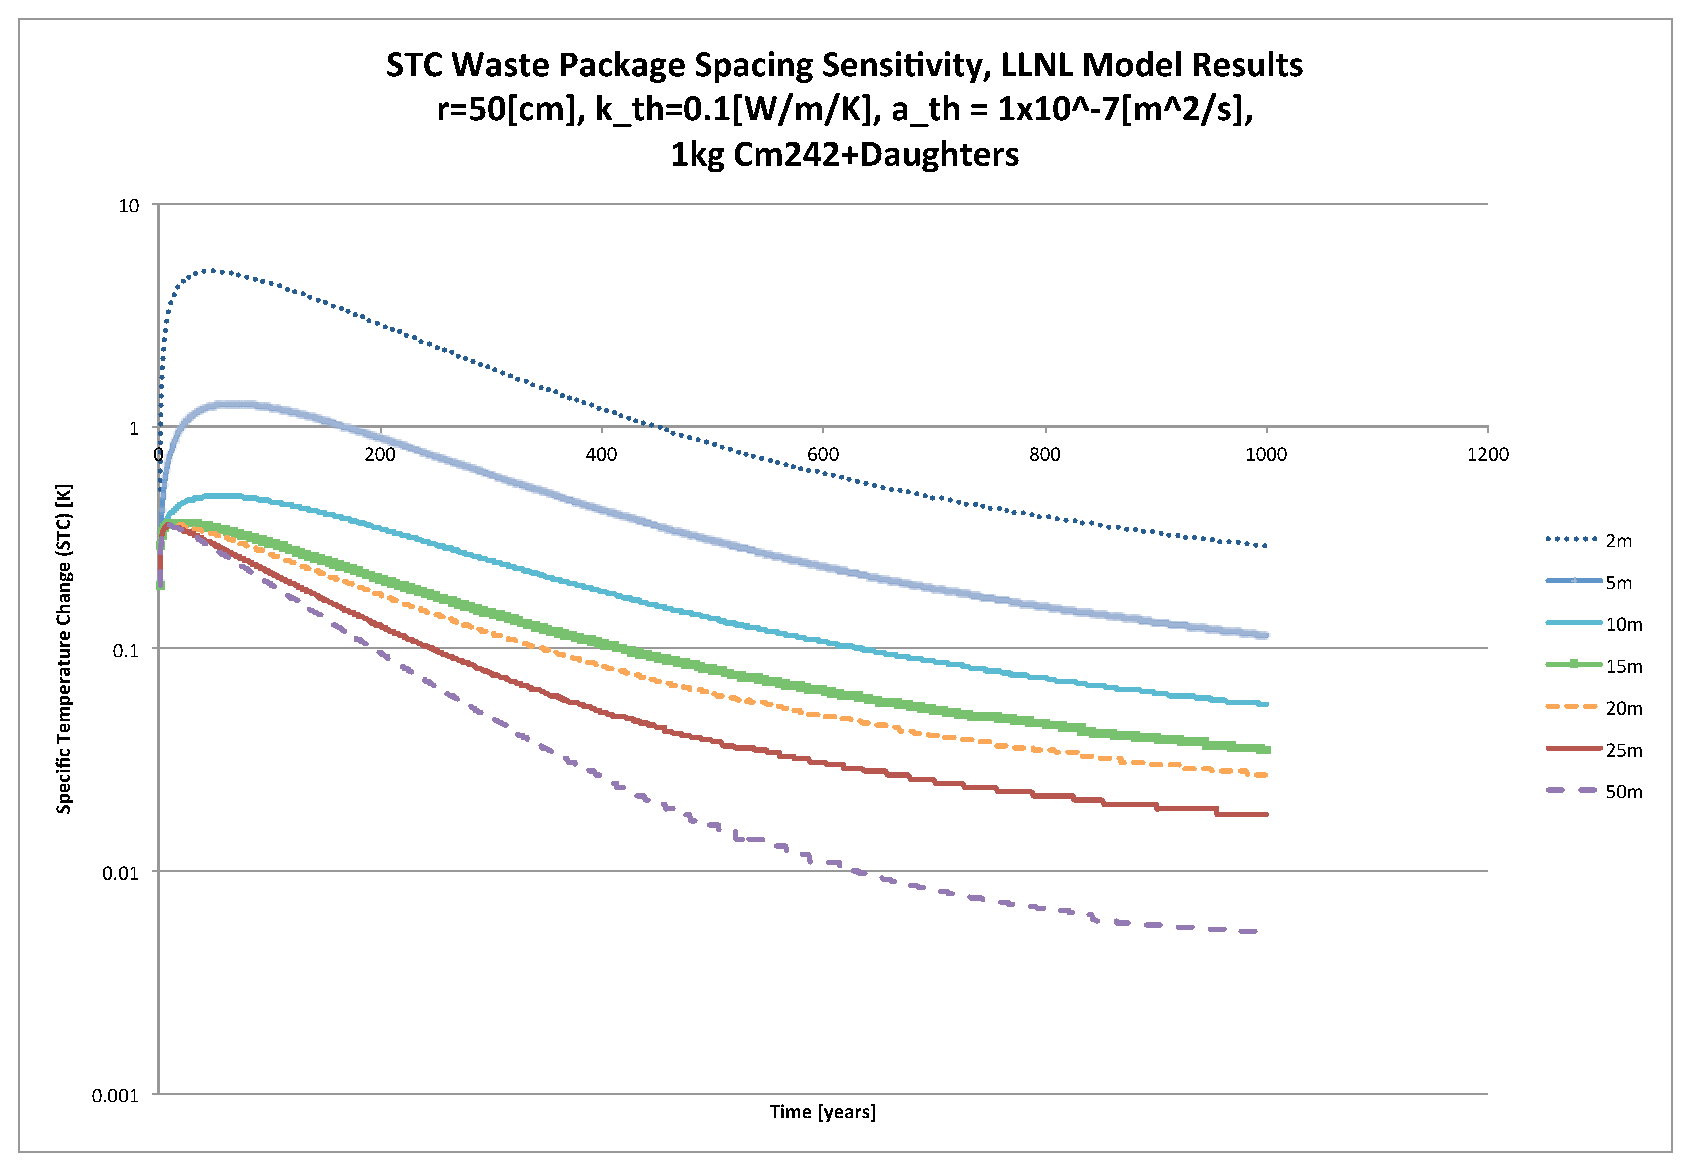
\includegraphics[width=\columnwidth]{./thermal_demonstration/spacing/Cm242spacing_sens.eps}
\end{center}
\caption[$K_{th}$ Sensitivity to $s$]{Increased waste package 
spacing decreases areal thermal energy deposition 
(here represented by \gls{STC}) in the near field (here $r_{calc} = 0.5m$).}
\label{fig:Cm242spacing_sens}
\end{figure}

Figure \ref{fig:Cm242spacing_sens} shows the trend in which increased waste package spacing of a medium decreases areal thermal energy 
deposition in the near field. This indicates that waste package spacing is 
an important parameter for repository concept design.

Similarly, the location of the limiting radius has a strong effect on the 
waste package loading limit, for a fixed limiting temperature. In Figure 
\ref{fig:Cm242r_lim_sens}, the trend is demonstrated in which increased limiting 
radius decreases the thermal energy contributing to the thermal limit. 


\begin{figure}[htbp!]
\begin{center}
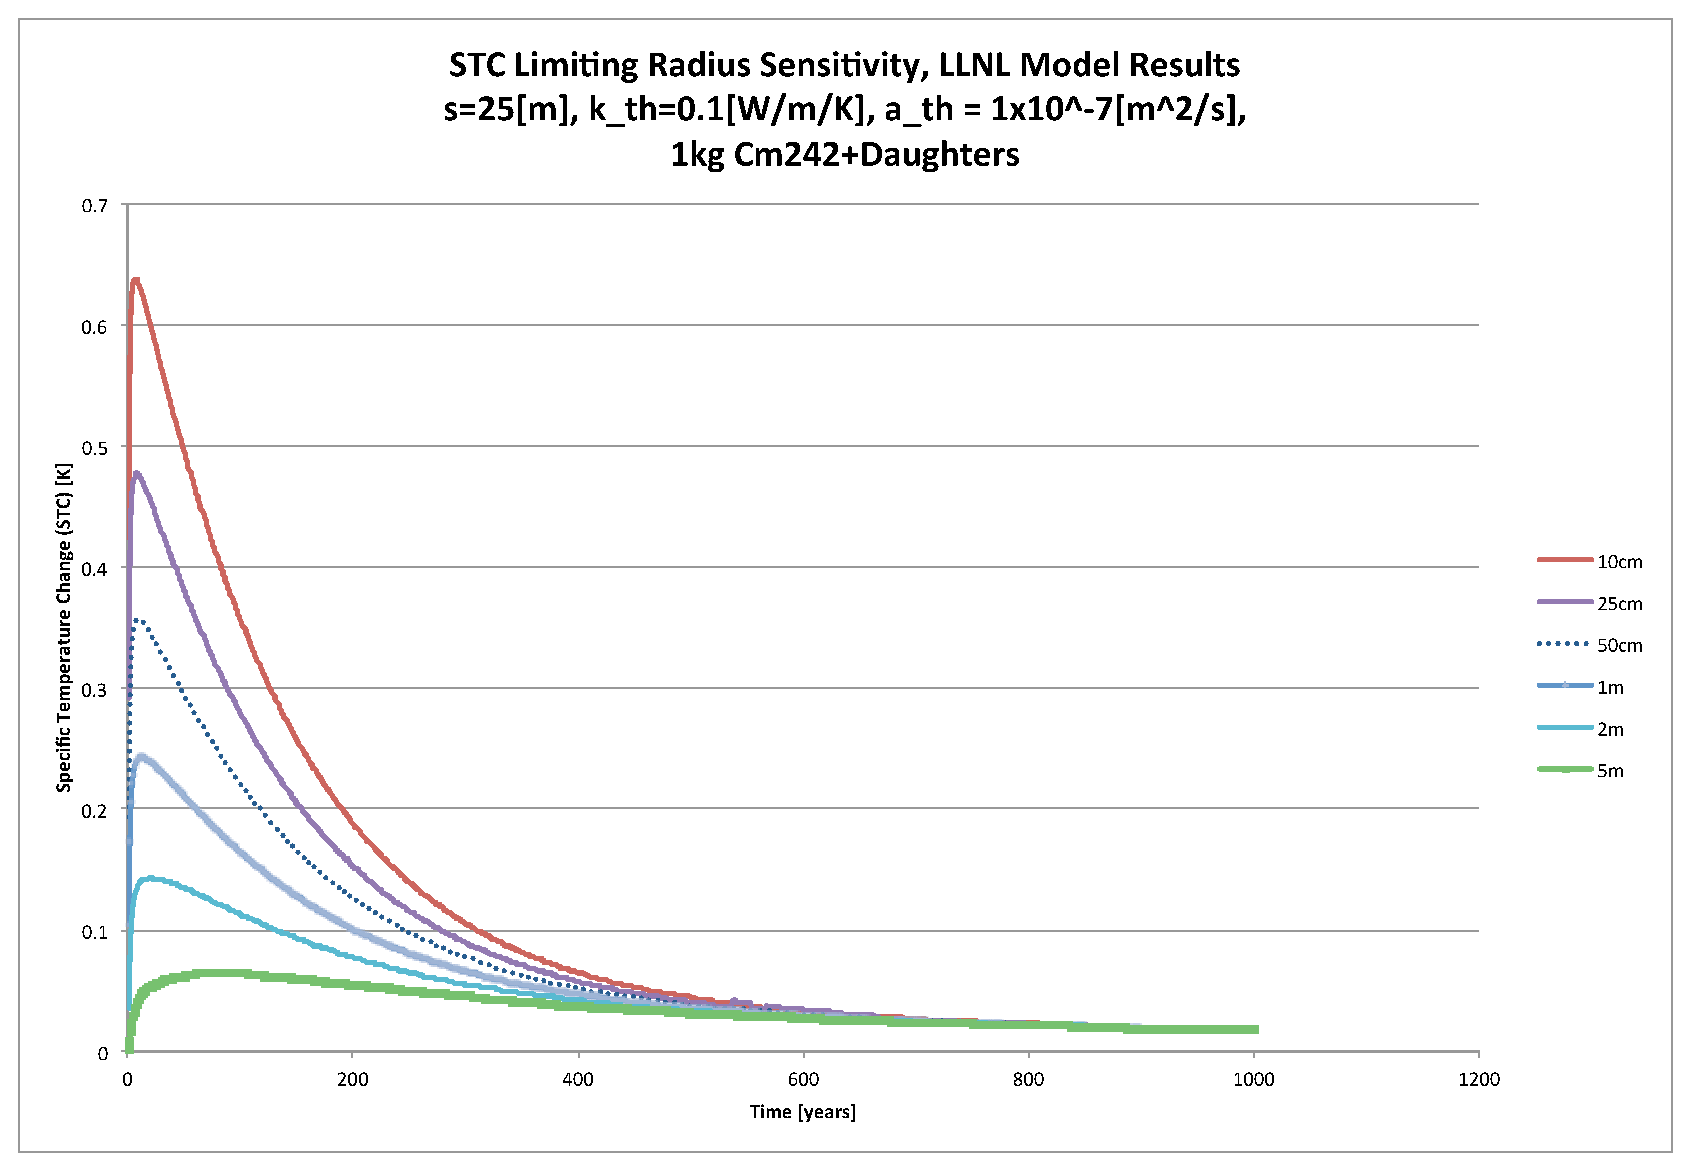
\includegraphics[width=\columnwidth]{./thermal_demonstration/spacing/Cm242r_lim_sens.eps}
\end{center}
\caption[$K_{th}$ Sensitivity to $r_{lim}$]{Increased limiting radius 
decreases thermal energy deposition contributing to the thermal limit
(here represented by \gls{STC}).}
\label{fig:Cm242r_lim_sens}
\end{figure}


\subsubsection{Cyder Results}

In a similar analysis, the thermal diffusivity was compared both with the 
spacing between waste packages and the limiting radius. 

Figure \ref{fig:rs} validates the trend noted above that 
increased waste package spacing in a repository concept decreases areal thermal energy deposition 
in the near field.  Additionally, analysis with the \Cyder STC database 
demonstrates the way in which the importance of $r_{lim}$, the limiting radius, 
impacts the maximum calculated temperature at that radius. 


\begin{figure}[htbp!]
\begin{center}
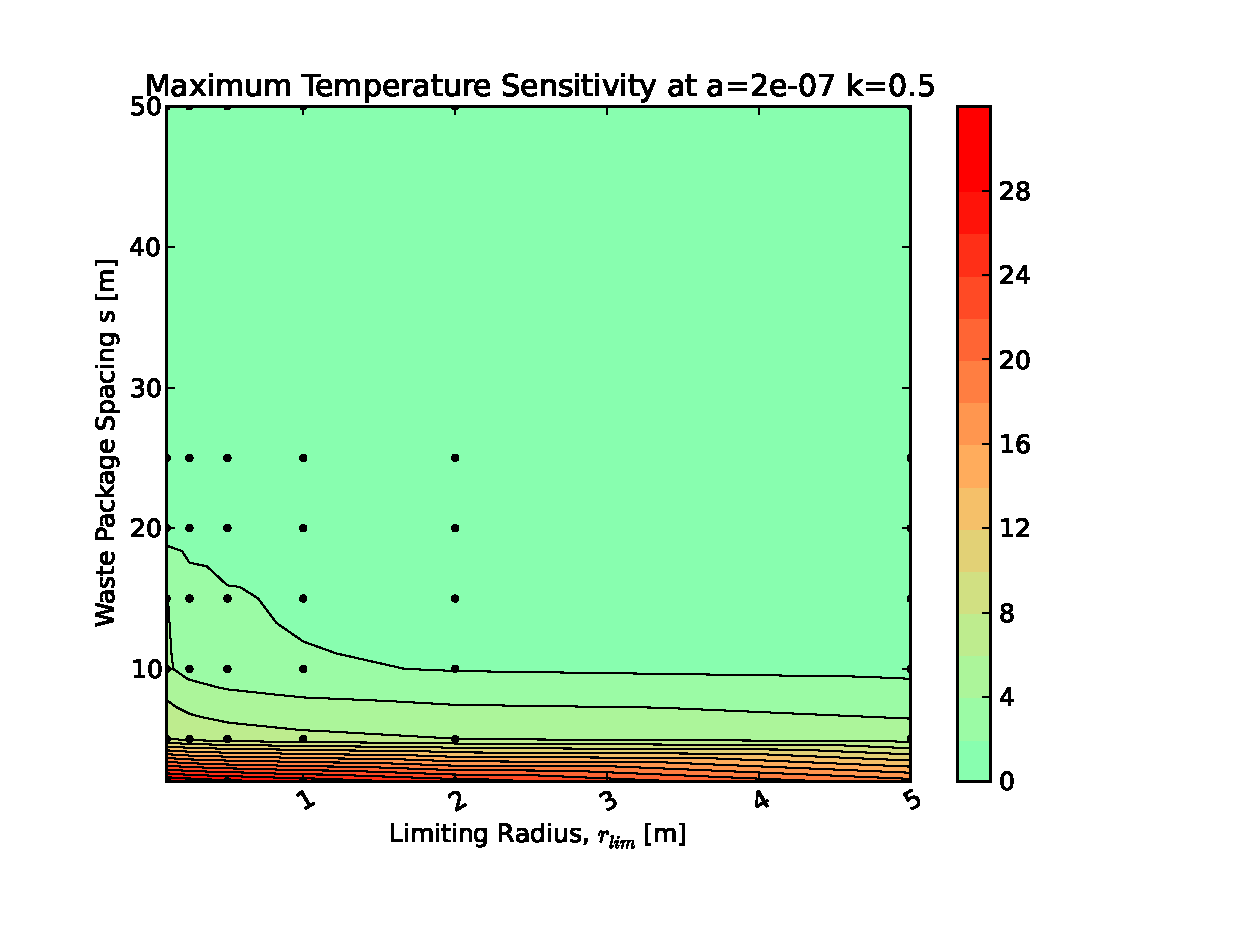
\includegraphics[width=\columnwidth]{./thermal_demonstration/spacing/rs.eps}
\end{center}
\caption[$\alpha_{th}$ vs. $r_{lim}$ Sensitivity in Cyder]
{Cyder results agree with 
those of the LLNL model. The importance of the limiting radius decreases with 
increased $K_{th}$. The above example thermal profile results from 10kg of 
$^{242}Cm$}
\label{fig:rs}
\end{figure}



